% !TEX root = ../main.tex
\chapter{Kế hoạch thực hiện, danh mục kiểm tra và hướng dẫn báo cáo}

\section{Danh mục kiểm tra lõi CRAG trước khi mở rộng}

\begin{infobox}{Mười bốn tiêu chí bắt buộc hoàn thành cho lõi CRAG}
\begin{enumerate}[label=\textbf{[\arabic*]}]
    \item Dữ liệu quy phạm pháp luật được thu thập từ nguồn chính thức của cơ quan nhà nước, có đầy đủ siêu dữ liệu hiệu lực và liên kết gốc.
    \item Phân tách đoạn trích theo đúng cấu trúc thứ bậc pháp lý (Chương $\to$ Điều $\to$ Khoản $\to$ Điểm).
    \item Hệ thống truy hồi lai (Dense BGE-M3 + Lexical BM25 + RRF + Cross-Encoder) hoạt động ổn định.
    \item Bộ đánh giá truy hồi phân loại độc lập và chính xác ba nhánh: Correct, Ambiguous và Incorrect.
    \item Hai ngưỡng $T_{low}$ và $T_{high}$ được tối ưu hóa bằng thực nghiệm quét lưới trên tập hiệu chuẩn riêng biệt.
    \item Nhánh Correct kích hoạt thành công cơ chế tinh lọc tri thức bóc tách các dải quy định cụ thể.
    \item Nhánh Incorrect kích hoạt viết lại truy vấn, tìm kiếm web có kiểm soát và lọc dải quy định ngoài.
    \item Nhánh Ambiguous kích hoạt đồng thời tinh lọc nội bộ và tìm kiếm web, hợp nhất bằng chứng đa nguồn.
    \item Bộ sinh chỉ được quyền sử dụng các đoạn trích đã vượt qua bộ lọc bằng chứng pháp lý.
    \item Bộ kiểm định trích dẫn phát hiện và chặn đứng mọi trích dẫn sai số hiệu hoặc không có thật.
    \item Sở hữu tập kiểm thử độc lập (40 câu hỏi) có gán nhãn căn cứ sự thật chi tiết.
    \item Thực hiện đo lường định lượng đầy đủ trên các hệ thống đối chứng $S_0, S_1, S_2, S_3$ và $S_4$.
    \item Phân tích ít nhất một trường hợp thất bại thực tế của hệ thống kèm nguyên nhân gốc rễ.
    \item Cam kết tuyệt đối không sử dụng bất kỳ số liệu giả định hay suy đoán nào trong báo cáo.
\end{enumerate}
\end{infobox}

\section{Lộ trình 17 giai đoạn triển khai dự án}

\begin{figure}[htbp]
    \centering
    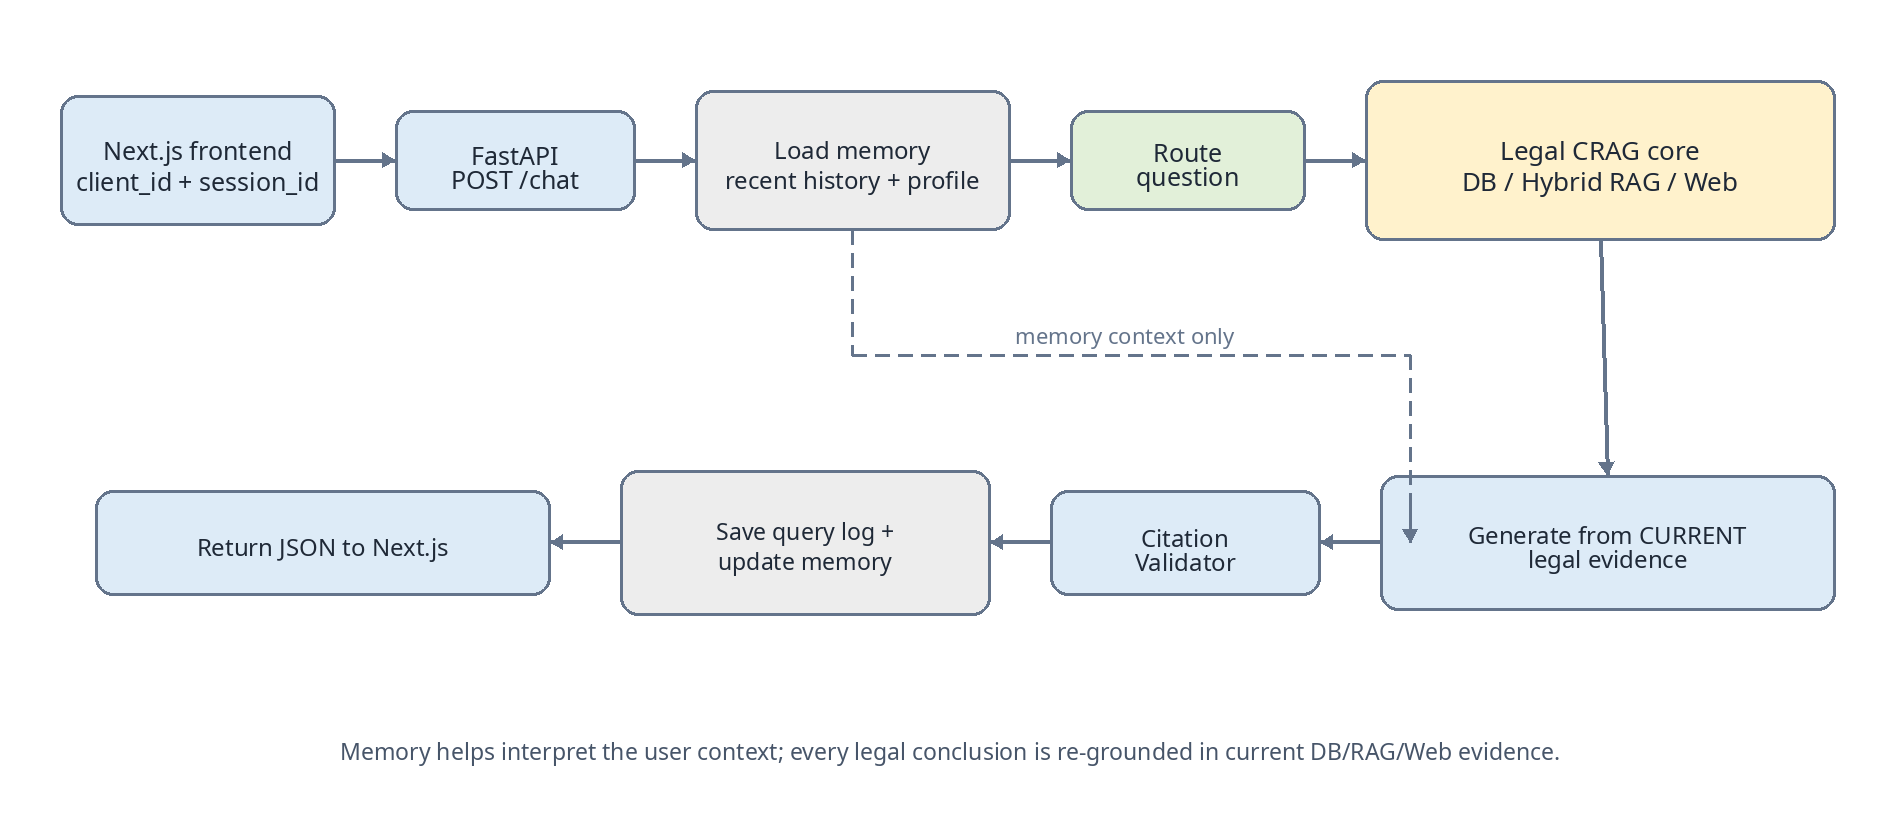
\includegraphics[width=\textwidth]{images/figure_3.png}
    \caption{Thứ tự thực hiện chuẩn mực: Ưu tiên dữ liệu, đo lường và lõi CRAG trước khi xây dựng giao diện người dùng.}
    \label{fig:implementation_flow}
\end{figure}

\begin{table}[htbp]
\centering
\caption{Kế hoạch thực hiện dự án theo 17 giai đoạn chuẩn hóa}
\label{tab:17_phases}
\renewcommand{\arraystretch}{1.2}
\rowcolors{2}{tablerowalt}{white}
\begin{tabularx}{\textwidth}{C{1.2cm} L{5.8cm} Y}
\toprule
\rowcolor{tableheader}\color{white}\textbf{Giai đoạn} & \color{white}\textbf{Công việc chi tiết} & \color{white}\textbf{Sản phẩm đầu ra (Deliverables)} \\
\midrule
1 & Xác định phạm vi và chính sách nguồn dữ liệu & Danh mục 50--100 văn bản pháp lý chính thống. \\
2 & Thu thập và bóc tách văn bản thô & Thư mục \texttt{data/raw} và \texttt{data/processed}. \\
3 & Chuẩn hóa siêu dữ liệu và quan hệ sửa đổi & Cơ sở dữ liệu SQLite \texttt{app.db} với các bảng quan hệ. \\
4 & Xây dựng tập hiệu chuẩn và tập kiểm thử & Tệp \texttt{calibration\_set.json} và \texttt{test\_set.json}. \\
5 & Cài đặt hệ thống truy hồi vector ngữ nghĩa & Kho vector ChromaDB với mô hình nhúng BGE-M3. \\
6 & Tích hợp BM25, thuật toán RRF và Reranker & Module truy hồi lai hoàn chỉnh. \\
7 & Cài đặt bộ đánh giá truy hồi và chọn ngưỡng & Cặp giá trị tối ưu $(T_{low}, T_{high})$ trên tập hiệu chuẩn. \\
8 & Hiện thực cơ chế tinh lọc tri thức & Nhánh Correct bóc tách các dải quy định cụ thể. \\
9 & Viết lại truy vấn và tìm kiếm web chính thống & Nhánh Incorrect với bộ lọc tên miền cho phép. \\
10 & Thuật toán hợp nhất và khử trùng lặp bằng chứng & Nhánh Ambiguous tích hợp đa nguồn. \\
11 & Xây dựng bộ kiểm định trích dẫn xác định & Module kiểm tra tính xác thực và hiệu lực trích dẫn. \\
12 & Hoàn thiện lõi tác tử LangGraph ReAct & Đồ thị StateGraph điều phối toàn bộ chu trình CRAG. \\
13 & Đo lường các hệ thống đối chứng và chỉ số RAGAS & Bảng số liệu thực nghiệm và vết thực thi LangFuse. \\
14 & Phát triển cổng API FastAPI và giao diện Next.js & Giao diện tra cứu và bảng trích dẫn căn cứ pháp luật. \\
15 & Tích hợp lịch sử hội thoại và hồ sơ ngữ nghĩa & Module lưu trữ phiên hội thoại SQLite. \\
16 & Đánh giá thử nghiệm A/B bộ nhớ & Báo cáo an toàn cách ly đạt Cross-client = 0. \\
17 & Hoàn thiện báo cáo kỹ thuật và trình diễn & Bản báo cáo LaTeX và mã nguồn nghiệm thu. \\
\bottomrule
\end{tabularx}
\end{table}

\section{Đề cương chi tiết 8 chương của báo cáo kỹ thuật}

Báo cáo kỹ thuật tốt nghiệp hoặc đồ án môn học chuẩn Thạc sĩ được phân bổ theo 8 chương:
\begin{enumerate}
    \item \textbf{Chương 1 -- Giới thiệu:} Bối cảnh ảo giác do truy hồi sai trong lĩnh vực pháp lý; bài toán trợ lý tuân thủ pháp lý doanh nghiệp; mục tiêu và năm câu hỏi nghiên cứu; phạm vi; các đóng góp chính của đề tài.
    \item \textbf{Chương 2 -- Cơ sở lý thuyết:} Tổng quan mô hình ngôn ngữ lớn nội bộ; tác tử AI có trạng thái; kiến trúc RAG cổ điển; truy hồi ngữ nghĩa với BGE-M3; BM25 và truy hồi lai; mô hình xếp hạng lại Cross-Encoder; LangGraph; nguyên lý Corrective RAG; khung đánh giá RAGAS; lý thuyết về bộ nhớ trong tác tử.
    \item \textbf{Chương 3 -- Phân tích và thiết kế hệ thống:} Đặc tả yêu cầu người dùng; kiến trúc ba tầng; luồng hoạt động chi tiết của LangGraph ReAct; thiết kế cơ sở dữ liệu pháp lý và quan hệ sửa đổi; mô hình trạng thái tác tử; chính sách kiểm soát nguồn web; thiết kế hệ thống kiểm định trích dẫn.
    \item \textbf{Chương 4 -- Chuẩn bị dữ liệu và tri thức:} Thu thập dữ liệu từ các cổng công quyền; kỹ thuật phân đoạn pháp lý; chuẩn hóa siêu dữ liệu; mô hình hóa lịch sử văn bản; lập chỉ mục vector Chroma và chỉ mục từ khóa BM25.
    \item \textbf{Chương 5 -- Xây dựng hệ thống tác tử:} Hiện thực truy hồi lai, RRF và Cross-Encoder; xây dựng bộ đánh giá với hai ngưỡng; chi tiết hóa ba nhánh CRAG; bộ sinh có cấu trúc JSON; kiểm định trích dẫn; kết nối FastAPI và giao diện Next.js; giám sát qua LangFuse.
    \item \textbf{Chương 6 -- Thiết kế thực nghiệm:} Phân tách tập hiệu chuẩn và tập kiểm thử độc lập; thiết kế các hệ thống đối chứng $S_0$--$S_4$; các phép thử phân tách thành phần; hệ thống các chỉ số truy hồi, điều hướng, chất lượng sinh và chuẩn mực pháp lý; quy trình quét lưới chọn ngưỡng.
    \item \textbf{Chương 7 -- Kết quả thực nghiệm và thảo luận:} Đánh giá chất lượng truy hồi; ma trận nhầm lẫn của bộ đánh giá; hiệu quả xử lý ba nhánh CRAG; phân tích các lượt gọi tìm kiếm ngoài; độ chính xác trích dẫn; phân tích các trường hợp thất bại thực tế.
    \item \textbf{Chương 8 -- Kết luận và hướng phát triển:} Đánh giá mức độ hoàn thành so với mục tiêu ban đầu; các hạn chế tồn đọng; đề xuất hướng mở rộng (đồ thị tri thức pháp lý, can thiệp của con người trong vòng lặp, tự động hóa cập nhật phiên bản).
\end{enumerate}
